\section{ME21B091}
\graphicspath{ {./ME21B091/} }
\begin{center}
\textbf{\large Variation of Electric resistance due to change in temperature}
\end{center}

\subsection{Introduction}
We are going to look into the variation of electric resistance due to the changes in temperature. Why does this happen? We will be looking into that in the next section.
\subsection{Variation of Electric resistance}
Variation in resistance happens due to the collisions between electrons and atoms of the medium. The electron flow/the current is resisted when other atoms are colliding with it and as the temperature increases, the collisions increase due to increase in energy of atoms and molecules. Thus resistance increases.

Electric resistance is shown linearly increasing with temperature for metals like copper for a moderate value for temperature
\begin{equation}
 R=R_0 (1+\alpha (T - T_0))
\end{equation}
Where,
\begin{center}
\begin{tabular}{|c|c|}
    \hline
    \textbf{Symbols and Letters used} & \textbf{Explanation} \\
    \hline
    \(R\) & Resistance at temperature \(T\) \\
    \hline
    \(R_0\) & Resistance at temperature \(T_0\) \\
    \hline
    \(\alpha\) & Temperature coefficient \\
    \hline
    \(T\) & Current temperature \\
    \hline
    \(T_0\) & Reference temperature \\
    \hline
     
\end{tabular}
\end{center}

\subsection{Graph of linear variation of resistance with temperature}

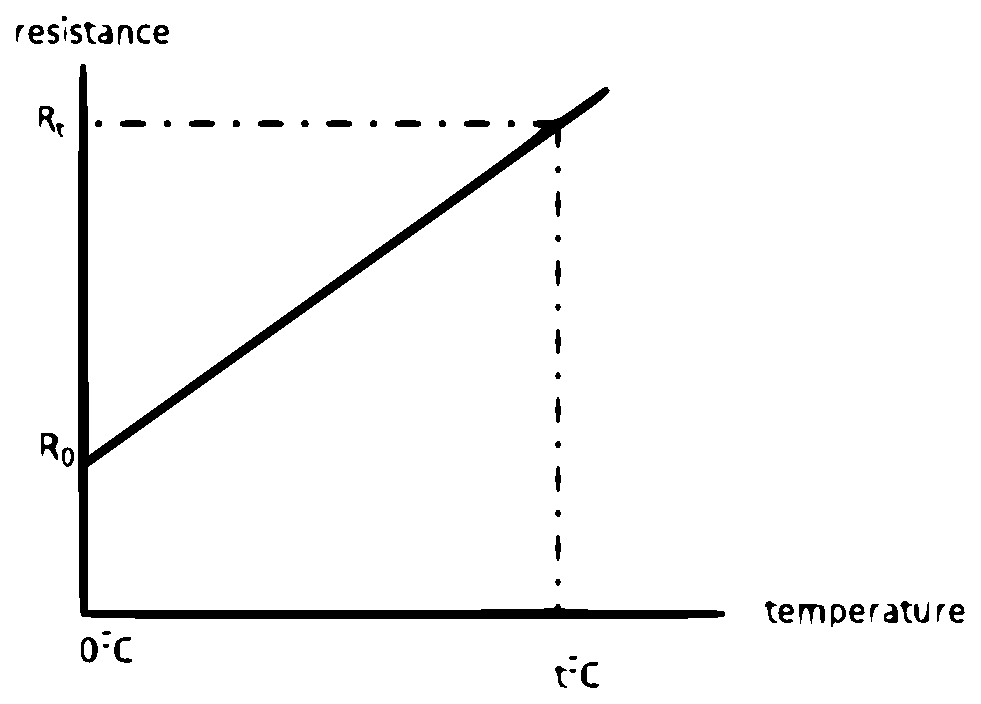
\includegraphics{hee.eps}


Image Source:
\href{https://electricstudents.blogspot.com/2017/06/effect-of-temperature-on-resistance-and.html}{Click Here}
    
\subsection{Further references}    

For further references see    


\url{https://www.electrical4u.com/resistance-variation-with-temperature/}
    
\url{https://byjus.com/physics/temperature-dependence-resistance/}
    
